\documentclass{article}\usepackage[]{graphicx}\usepackage[]{color}
%% maxwidth is the original width if it is less than linewidth
%% otherwise use linewidth (to make sure the graphics do not exceed the margin)
\makeatletter
\def\maxwidth{ %
  \ifdim\Gin@nat@width>\linewidth
    \linewidth
  \else
    \Gin@nat@width
  \fi
}
\makeatother

\definecolor{fgcolor}{rgb}{0.345, 0.345, 0.345}
\newcommand{\hlnum}[1]{\textcolor[rgb]{0.686,0.059,0.569}{#1}}%
\newcommand{\hlstr}[1]{\textcolor[rgb]{0.192,0.494,0.8}{#1}}%
\newcommand{\hlcom}[1]{\textcolor[rgb]{0.678,0.584,0.686}{\textit{#1}}}%
\newcommand{\hlopt}[1]{\textcolor[rgb]{0,0,0}{#1}}%
\newcommand{\hlstd}[1]{\textcolor[rgb]{0.345,0.345,0.345}{#1}}%
\newcommand{\hlkwa}[1]{\textcolor[rgb]{0.161,0.373,0.58}{\textbf{#1}}}%
\newcommand{\hlkwb}[1]{\textcolor[rgb]{0.69,0.353,0.396}{#1}}%
\newcommand{\hlkwc}[1]{\textcolor[rgb]{0.333,0.667,0.333}{#1}}%
\newcommand{\hlkwd}[1]{\textcolor[rgb]{0.737,0.353,0.396}{\textbf{#1}}}%

\usepackage{framed}
\makeatletter
\newenvironment{kframe}{%
 \def\at@end@of@kframe{}%
 \ifinner\ifhmode%
  \def\at@end@of@kframe{\end{minipage}}%
  \begin{minipage}{\columnwidth}%
 \fi\fi%
 \def\FrameCommand##1{\hskip\@totalleftmargin \hskip-\fboxsep
 \colorbox{shadecolor}{##1}\hskip-\fboxsep
     % There is no \\@totalrightmargin, so:
     \hskip-\linewidth \hskip-\@totalleftmargin \hskip\columnwidth}%
 \MakeFramed {\advance\hsize-\width
   \@totalleftmargin\z@ \linewidth\hsize
   \@setminipage}}%
 {\par\unskip\endMakeFramed%
 \at@end@of@kframe}
\makeatother

\definecolor{shadecolor}{rgb}{.97, .97, .97}
\definecolor{messagecolor}{rgb}{0, 0, 0}
\definecolor{warningcolor}{rgb}{1, 0, 1}
\definecolor{errorcolor}{rgb}{1, 0, 0}
\newenvironment{knitrout}{}{} % an empty environment to be redefined in TeX

\usepackage{alltt}
\usepackage{geometry}
\usepackage{amsmath}
\usepackage{lscape}
\geometry{verbose,tmargin=2.5cm,bmargin=2.5cm,lmargin=2.5cm,rmargin=2.5cm}
\IfFileExists{upquote.sty}{\usepackage{upquote}}{}
\begin{document}




\title{Messina E3: Messina vs ? on APGI}
\maketitle


%%%%%%%%%%%%%%%%%%%%%%%%%%%%%%%%%%%%%%%%%%%%%%%%%%%%%%%%%%%%%%%%%%%%%%
% LIBRARIES
%%%%%%%%%%%%%%%%%%%%%%%%%%%%%%%%%%%%%%%%%%%%%%%%%%%%%%%%%%%%%%%%%%%%%%
\section{Preparation}
\begin{knitrout}
\definecolor{shadecolor}{rgb}{0.969, 0.969, 0.969}\color{fgcolor}\begin{kframe}
\begin{alltt}
\hlkwd{library}\hlstd{(plyr)}
\hlkwd{library}\hlstd{(ggplot2)}
\end{alltt}


{\ttfamily\noindent\itshape\color{messagecolor}{\#\# Loading required package: methods}}\begin{alltt}
\hlkwd{library}\hlstd{(messina)}
\end{alltt}


{\ttfamily\noindent\itshape\color{messagecolor}{\#\# Loading required package: survival\\\#\# Loading required package: splines}}\begin{alltt}
\hlkwd{library}\hlstd{(maxstat)}
\hlkwd{library}\hlstd{(doMC)}
\end{alltt}


{\ttfamily\noindent\itshape\color{messagecolor}{\#\# Loading required package: foreach\\\#\# Loading required package: iterators\\\#\# Loading required package: parallel}}\begin{alltt}
\hlstd{paropts} \hlkwb{=} \hlkwd{list}\hlstd{(}\hlkwc{.options.multicore} \hlstd{=} \hlkwd{list}\hlstd{(}\hlkwc{preschedule} \hlstd{=} \hlnum{FALSE}\hlstd{))}
\end{alltt}
\end{kframe}
\end{knitrout}


\section{Data preparation}
\begin{knitrout}
\definecolor{shadecolor}{rgb}{0.969, 0.969, 0.969}\color{fgcolor}\begin{kframe}
\begin{alltt}
\hlkwd{load}\hlstd{(}\hlstr{"../biosurv/data/07_data_for_SIS.rda"}\hlstd{)}
\hlstd{APGI.x} \hlkwb{=} \hlstd{x.diag_dsd}
\hlstd{APGI.y} \hlkwb{=} \hlstd{y.diag_dsd}
\hlstd{APGI.samps} \hlkwb{=} \hlstd{samps.diag_dsd}
\hlstd{APGI.feats} \hlkwb{=} \hlkwd{data.frame}\hlstd{(}\hlkwc{symbol} \hlstd{=} \hlkwd{rownames}\hlstd{(APGI.x))}

\hlstd{temp} \hlkwb{=} \hlnum{NA}
\hlstd{temp} \hlkwb{=} \hlkwd{ls}\hlstd{()}
\hlkwd{rm}\hlstd{(}\hlkwc{list} \hlstd{= temp[}\hlopt{!}\hlstd{(temp} \hlopt \hlkwd{c}\hlstd{(}\hlstr{"APGI.x"}\hlstd{,} \hlstr{"APGI.y"}\hlstd{,} \hlstr{"APGI.samps"}\hlstd{,} \hlstr{"APGI.feats"}\hlstd{))])}

\hlkwd{load}\hlstd{(}\hlstr{"../biosurv/data/15_validation.rda"}\hlstd{)}
\hlkwd{rm}\hlstd{(GSE28735.lingex, GSE21501.lingex)}
\hlstd{GSE28735.x} \hlkwb{=} \hlstd{GSE28735.gex}
\hlstd{GSE21501.x} \hlkwb{=} \hlstd{GSE21501.gex}
\hlstd{GSE28735.feats} \hlkwb{=} \hlstd{GSE28735.feat}
\hlstd{GSE21501.feats} \hlkwb{=} \hlstd{GSE21501.feat}
\hlkwd{rm}\hlstd{(GSE28735.gex, GSE21501.gex, GSE28735.feat, GSE21501.feat)}

\hlkwd{load}\hlstd{(}\hlstr{"../biosurv/data/validation/tcga-clin-gex.20141118.rda"}\hlstd{)}
\hlstd{TCGA.x} \hlkwb{=} \hlstd{data.merged}\hlopt{$}\hlstd{paad}\hlopt{$}\hlstd{gex}\hlopt{$}\hlstd{illuminahiseq_rnaseqv2}
\hlkwd{rownames}\hlstd{(TCGA.x)} \hlkwb{=} \hlkwd{gsub}\hlstd{(}\hlstr{"\textbackslash{}\textbackslash{}|.*"}\hlstd{,} \hlstr{""}\hlstd{,} \hlkwd{rownames}\hlstd{(TCGA.x))}
\hlstd{TCGA.x} \hlkwb{=} \hlstd{TCGA.x[}\hlkwd{rownames}\hlstd{(TCGA.x)} \hlopt{!=} \hlstr{"?"}\hlstd{,]}
\hlstd{TCGA.x} \hlkwb{=} \hlkwd{log2}\hlstd{(TCGA.x} \hlopt{+} \hlnum{1}\hlstd{)}
\hlstd{temp.time} \hlkwb{=} \hlkwd{as.numeric}\hlstd{(}\hlkwd{as.character}\hlstd{(data.merged}\hlopt{$}\hlstd{paad}\hlopt{$}\hlstd{clin}\hlopt{$}\hlstd{days_to_death))}
\hlstd{temp.time[}\hlkwd{is.na}\hlstd{(temp.time)]} \hlkwb{=} \hlkwd{as.numeric}\hlstd{(}\hlkwd{as.character}\hlstd{(data.merged}\hlopt{$}\hlstd{paad}\hlopt{$}\hlstd{clin}\hlopt{$}\hlstd{days_to_last_followup[}\hlkwd{is.na}\hlstd{(temp.time)]))}
\hlstd{TCGA.y} \hlkwb{=} \hlkwd{Surv}\hlstd{(temp.time, data.merged}\hlopt{$}\hlstd{paad}\hlopt{$}\hlstd{clin}\hlopt{$}\hlstd{vital_status} \hlopt{==} \hlstr{"Dead"}\hlstd{)}
\hlstd{TCGA.feats} \hlkwb{=} \hlkwd{data.frame}\hlstd{(}\hlkwc{symbol} \hlstd{=} \hlkwd{rownames}\hlstd{(TCGA.x))}
\hlkwd{rm}\hlstd{(data.merged)}

\hlstd{keepMostVariableGeneMeasurement} \hlkwb{=} \hlkwa{function}\hlstd{(}\hlkwc{gex}\hlstd{,} \hlkwc{feats}\hlstd{,} \hlkwc{ids}\hlstd{)}
\hlstd{\{}
        \hlstd{sds} \hlkwb{=} \hlkwd{apply}\hlstd{(gex,} \hlnum{1}\hlstd{, sd,} \hlkwc{na.rm} \hlstd{=} \hlnum{TRUE}\hlstd{)}
        \hlstd{perm} \hlkwb{=} \hlkwd{order}\hlstd{(}\hlopt{-}\hlstd{sds)}
        \hlstd{gex} \hlkwb{=} \hlstd{gex[perm,,}\hlkwc{drop} \hlstd{=} \hlnum{FALSE}\hlstd{]}
        \hlstd{feats} \hlkwb{=} \hlstd{feats[perm,,}\hlkwc{drop} \hlstd{=} \hlnum{FALSE}\hlstd{]}
        \hlstd{ids} \hlkwb{=} \hlstd{ids[perm]}
        \hlstd{drop} \hlkwb{=} \hlkwd{duplicated}\hlstd{(ids)} \hlopt{|} \hlkwd{is.null}\hlstd{(ids)}
        \hlstd{gex} \hlkwb{=} \hlstd{gex[}\hlopt{!}\hlstd{drop,,}\hlkwc{drop} \hlstd{=} \hlnum{FALSE}\hlstd{]}
        \hlstd{feats} \hlkwb{=} \hlstd{feats[}\hlopt{!}\hlstd{drop,,}\hlkwc{drop} \hlstd{=} \hlnum{FALSE}\hlstd{]}
        \hlstd{ids} \hlkwb{=} \hlstd{ids[}\hlopt{!}\hlstd{drop]}
        \hlkwd{list}\hlstd{(}\hlkwc{gex} \hlstd{= gex,} \hlkwc{feats} \hlstd{= feats,} \hlkwc{ids} \hlstd{= ids)}
\hlstd{\}}

\hlcom{# Now moved to the validation function}
\hlcom{# regularizeX = function(x)}
\hlcom{# \{}
\hlcom{# 	require(robustbase)}
\hlcom{# 	location = apply(x, 1, median, na.rm = TRUE)}
\hlcom{# 	scale = apply(x, 1, scaleTau2, na.rm = TRUE)}
\hlcom{# 	(x - location) / scale}
\hlcom{# \}}

\hlstd{temp} \hlkwb{=} \hlkwd{keepMostVariableGeneMeasurement}\hlstd{(APGI.x, APGI.feats, APGI.feats}\hlopt{$}\hlstd{symbol)}
\hlstd{APGI.x} \hlkwb{=} \hlstd{temp}\hlopt{$}\hlstd{gex}
\hlstd{APGI.feats} \hlkwb{=} \hlstd{temp}\hlopt{$}\hlstd{feats}
\hlstd{temp} \hlkwb{=} \hlkwd{keepMostVariableGeneMeasurement}\hlstd{(GSE28735.x, GSE28735.feats, GSE28735.feats}\hlopt{$}\hlstd{Gene.symbol)}
\hlstd{GSE28735.x} \hlkwb{=} \hlstd{temp}\hlopt{$}\hlstd{gex}
\hlstd{GSE28735.feats} \hlkwb{=} \hlstd{temp}\hlopt{$}\hlstd{feats}
\hlstd{temp} \hlkwb{=} \hlkwd{keepMostVariableGeneMeasurement}\hlstd{(GSE21501.x, GSE21501.feats, GSE21501.feats}\hlopt{$}\hlstd{Gene.symbol)}
\hlstd{GSE21501.x} \hlkwb{=} \hlstd{temp}\hlopt{$}\hlstd{gex}
\hlstd{GSE21501.feats} \hlkwb{=} \hlstd{temp}\hlopt{$}\hlstd{feats}

\hlstd{GSE28735.y} \hlkwb{=} \hlkwd{Surv}\hlstd{(GSE28735.samp}\hlopt{$}\hlstd{time, GSE28735.samp}\hlopt{$}\hlstd{event)}
\hlstd{GSE21501.y} \hlkwb{=} \hlkwd{Surv}\hlstd{(GSE21501.samp}\hlopt{$}\hlstd{time, GSE21501.samp}\hlopt{$}\hlstd{event)}

\hlcom{# APGI.xreg = regularizeX(APGI.x)}
\hlcom{# GSE28735.xreg = regularizeX(GSE28735.x)		# This one validated for survsigs}
\hlcom{# GSE21501.xreg = regularizeX(GSE21501.x)}
\end{alltt}
\end{kframe}
\end{knitrout}


\begin{knitrout}
\definecolor{shadecolor}{rgb}{0.969, 0.969, 0.969}\color{fgcolor}\begin{kframe}
\begin{alltt}
\hlcom{# Temporary testing measure.  Probably will be used in real application, but somewhat defeats}
\hlcom{# the whole purpose of Messina for testing, so should be removed when comparing vs other methods.}
\hlcom{# temp.sel = apply(APGI.x, 1, sd) >= 1 & grepl("^D", rownames(APGI.x))}
\hlcom{# APGI.x = APGI.x[temp.sel,,drop = FALSE]}
\hlcom{# APGI.feats = APGI.feats[temp.sel,,drop = FALSE]}

\hlcom{# messinaSurv(APGI.x, APGI.y, messinaSurvObj.CoxCoef(round(log(2), 3)), parallel = TRUE, silent = FALSE, seed = 20150321)}
\hlcom{# messinaSurv(APGI.x, APGI.y, messinaSurvObj.Tau(0.6), parallel = TRUE, silent = FALSE, seed = 20150321)}
\hlcom{# messinaSurv(APGI.x, APGI.y, messinaSurvObj.RelTau(0.7), parallel = TRUE, silent = FALSE, seed = 20150321)}

\hlkwd{registerDoMC}\hlstd{(}\hlnum{32}\hlstd{)}

\hlkwd{library}\hlstd{(plyr)}
\hlstd{APGI.messina.cc2} \hlkwb{=} \hlkwd{messinaSurv}\hlstd{(APGI.x, APGI.y,} \hlkwd{messinaSurvObj.CoxCoef}\hlstd{(}\hlkwd{round}\hlstd{(}\hlkwd{log}\hlstd{(}\hlnum{2}\hlstd{),} \hlnum{3}\hlstd{)),} \hlkwc{parallel} \hlstd{=} \hlnum{TRUE}\hlstd{,} \hlkwc{silent} \hlstd{=} \hlnum{FALSE}\hlstd{,} \hlkwc{seed} \hlstd{=} \hlnum{20150321}\hlstd{)}
\end{alltt}


{\ttfamily\noindent\itshape\color{messagecolor}{\#\# Performance bootstrapping...\\\#\# Final training...}}\begin{alltt}
\hlstd{APGI.messina.cc3} \hlkwb{=} \hlkwd{messinaSurv}\hlstd{(APGI.x, APGI.y,} \hlkwd{messinaSurvObj.CoxCoef}\hlstd{(}\hlkwd{round}\hlstd{(}\hlkwd{log}\hlstd{(}\hlnum{3}\hlstd{),} \hlnum{3}\hlstd{)),} \hlkwc{parallel} \hlstd{=} \hlnum{TRUE}\hlstd{,} \hlkwc{silent} \hlstd{=} \hlnum{FALSE}\hlstd{,} \hlkwc{seed} \hlstd{=} \hlnum{20150321}\hlstd{)}
\end{alltt}


{\ttfamily\noindent\itshape\color{messagecolor}{\#\# Performance bootstrapping...\\\#\# Final training...}}\begin{alltt}
\hlstd{APGI.messina.tau6} \hlkwb{=} \hlkwd{messinaSurv}\hlstd{(APGI.x, APGI.y,} \hlkwd{messinaSurvObj.Tau}\hlstd{(}\hlnum{0.6}\hlstd{),} \hlkwc{parallel} \hlstd{=} \hlnum{TRUE}\hlstd{,} \hlkwc{silent} \hlstd{=} \hlnum{FALSE}\hlstd{,} \hlkwc{seed} \hlstd{=} \hlnum{20150321}\hlstd{)}
\end{alltt}


{\ttfamily\noindent\itshape\color{messagecolor}{\#\# Performance bootstrapping...\\\#\# Final training...}}\begin{alltt}
\hlstd{APGI.messina.tau7} \hlkwb{=} \hlkwd{messinaSurv}\hlstd{(APGI.x, APGI.y,} \hlkwd{messinaSurvObj.Tau}\hlstd{(}\hlnum{0.7}\hlstd{),} \hlkwc{parallel} \hlstd{=} \hlnum{TRUE}\hlstd{,} \hlkwc{silent} \hlstd{=} \hlnum{FALSE}\hlstd{,} \hlkwc{seed} \hlstd{=} \hlnum{20150321}\hlstd{)}
\end{alltt}


{\ttfamily\noindent\itshape\color{messagecolor}{\#\# Performance bootstrapping...\\\#\# Final training...}}\begin{alltt}
\hlstd{APGI.messina} \hlkwb{=} \hlstd{APGI.messina.cc2}
\hlstd{APGI.maxstat} \hlkwb{=} \hlkwd{alply}\hlstd{(APGI.x,} \hlnum{1}\hlstd{,} \hlkwa{function}\hlstd{(}\hlkwc{x1}\hlstd{) \{}
        \hlstd{data} \hlkwb{=} \hlkwd{data.frame}\hlstd{(}\hlkwc{time} \hlstd{= APGI.y[,}\hlnum{1}\hlstd{],} \hlkwc{event} \hlstd{= APGI.y[,}\hlnum{2}\hlstd{],} \hlkwc{x} \hlstd{= x1)}
        \hlstd{test} \hlkwb{=} \hlkwd{try}\hlstd{(}\hlkwd{maxstat.test}\hlstd{(}\hlkwd{Surv}\hlstd{(time, event)} \hlopt{~} \hlstd{x,} \hlkwc{data} \hlstd{= data,} \hlkwc{smethod} \hlstd{=} \hlstr{"LogRank"}\hlstd{,} \hlkwc{pmethod} \hlstd{=} \hlstr{"HL"}\hlstd{))}
        \hlstd{result} \hlkwb{=} \hlkwd{list}\hlstd{(}\hlkwc{p.value} \hlstd{=} \hlnum{NA}\hlstd{,} \hlkwc{threshold} \hlstd{=} \hlnum{NA}\hlstd{)}
        \hlkwa{if} \hlstd{(}\hlkwd{class}\hlstd{(test)} \hlopt{!=} \hlstr{"try-error"}\hlstd{)}
        \hlstd{\{}
                \hlstd{result}\hlopt{$}\hlstd{p.value} \hlkwb{=} \hlstd{test}\hlopt{$}\hlstd{p.value}
                \hlstd{result}\hlopt{$}\hlstd{threshold} \hlkwb{=} \hlstd{test}\hlopt{$}\hlstd{estimate}
        \hlstd{\}}
        \hlstd{result}
\hlstd{\},} \hlkwc{.parallel} \hlstd{=} \hlnum{TRUE}\hlstd{)}
\end{alltt}
\end{kframe}
\end{knitrout}


\begin{knitrout}
\definecolor{shadecolor}{rgb}{0.969, 0.969, 0.969}\color{fgcolor}\begin{kframe}
\begin{alltt}
\hlkwd{print}\hlstd{(}\hlkwd{dim}\hlstd{(APGI.x))}
\end{alltt}
\begin{verbatim}
## [1] 13000   110
\end{verbatim}
\begin{alltt}
\hlkwd{hist}\hlstd{(APGI.messina}\hlopt{@}\hlkwc{fits}\hlopt{@}\hlkwc{summary}\hlopt{$}\hlstd{margin,} \hlkwc{main} \hlstd{=} \hlstr{""}\hlstd{,} \hlkwc{xlab} \hlstd{=} \hlstr{""}\hlstd{)}
\end{alltt}
\end{kframe}

{\centering 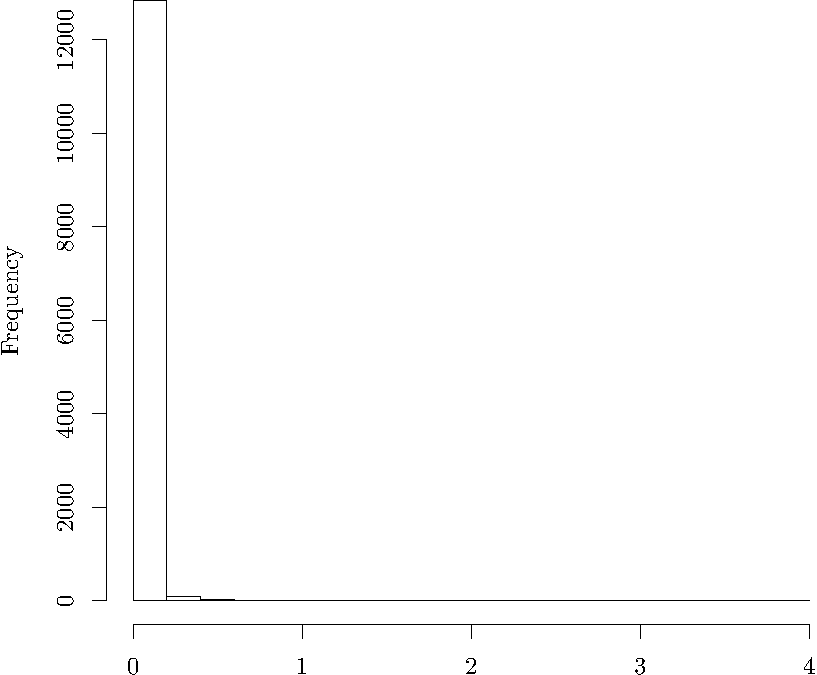
\includegraphics[width=\maxwidth]{figure/07-E3-E3-summary-1} 

}


\begin{kframe}\begin{alltt}
\hlkwd{hist}\hlstd{(APGI.messina}\hlopt{@}\hlkwc{fits}\hlopt{@}\hlkwc{summary}\hlopt{$}\hlstd{margin[APGI.messina}\hlopt{@}\hlkwc{fits}\hlopt{@}\hlkwc{summary}\hlopt{$}\hlstd{passed} \hlopt{==} \hlnum{TRUE}\hlstd{],} \hlkwc{main} \hlstd{=} \hlstr{""}\hlstd{,} \hlkwc{xlab} \hlstd{=} \hlstr{""}\hlstd{)}
\end{alltt}
\end{kframe}

{\centering 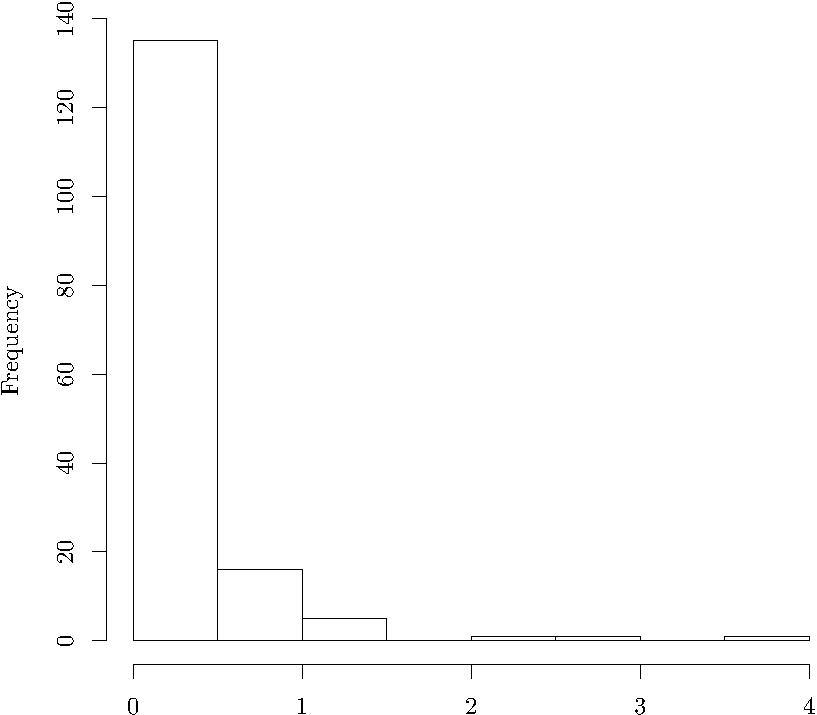
\includegraphics[width=\maxwidth]{figure/07-E3-E3-summary-2} 

}


\begin{kframe}\begin{alltt}
\hlkwd{sum}\hlstd{(APGI.messina}\hlopt{@}\hlkwc{fits}\hlopt{@}\hlkwc{summary}\hlopt{$}\hlstd{passed} \hlopt{==} \hlnum{TRUE}\hlstd{)}
\end{alltt}
\begin{verbatim}
## [1] 159
\end{verbatim}
\begin{alltt}
\hlkwd{mean}\hlstd{(APGI.messina}\hlopt{@}\hlkwc{fits}\hlopt{@}\hlkwc{summary}\hlopt{$}\hlstd{passed} \hlopt{==} \hlnum{TRUE}\hlstd{)}
\end{alltt}
\begin{verbatim}
## [1] 0.01223
\end{verbatim}
\begin{alltt}
\hlkwd{sum}\hlstd{(APGI.messina}\hlopt{@}\hlkwc{fits}\hlopt{@}\hlkwc{summary}\hlopt{$}\hlstd{margin} \hlopt{>=} \hlnum{1}\hlstd{)}
\end{alltt}
\begin{verbatim}
## [1] 11
\end{verbatim}
\begin{alltt}
\hlkwd{mean}\hlstd{(APGI.messina}\hlopt{@}\hlkwc{fits}\hlopt{@}\hlkwc{summary}\hlopt{$}\hlstd{margin} \hlopt{>=} \hlnum{1}\hlstd{)}
\end{alltt}
\begin{verbatim}
## [1] 0.0008462
\end{verbatim}
\begin{alltt}
\hlkwd{sum}\hlstd{(APGI.messina}\hlopt{@}\hlkwc{fits}\hlopt{@}\hlkwc{summary}\hlopt{$}\hlstd{margin} \hlopt{>=} \hlnum{1} \hlopt{&} \hlstd{APGI.messina}\hlopt{@}\hlkwc{fits}\hlopt{@}\hlkwc{summary}\hlopt{$}\hlstd{passed} \hlopt{==} \hlnum{TRUE}\hlstd{)}
\end{alltt}
\begin{verbatim}
## [1] 8
\end{verbatim}
\begin{alltt}
\hlkwd{mean}\hlstd{(APGI.messina}\hlopt{@}\hlkwc{fits}\hlopt{@}\hlkwc{summary}\hlopt{$}\hlstd{margin} \hlopt{>=} \hlnum{1} \hlopt{&} \hlstd{APGI.messina}\hlopt{@}\hlkwc{fits}\hlopt{@}\hlkwc{summary}\hlopt{$}\hlstd{passed} \hlopt{==} \hlnum{TRUE}\hlstd{)}
\end{alltt}
\begin{verbatim}
## [1] 0.0006154
\end{verbatim}
\begin{alltt}
\hlkwd{hist}\hlstd{(}\hlkwd{sapply}\hlstd{(APGI.maxstat,} \hlkwa{function}\hlstd{(}\hlkwc{x}\hlstd{) x}\hlopt{$}\hlstd{p.value),} \hlkwc{main} \hlstd{=} \hlstr{""}\hlstd{,} \hlkwc{xlab} \hlstd{=} \hlstr{""}\hlstd{)}
\end{alltt}
\end{kframe}

{\centering 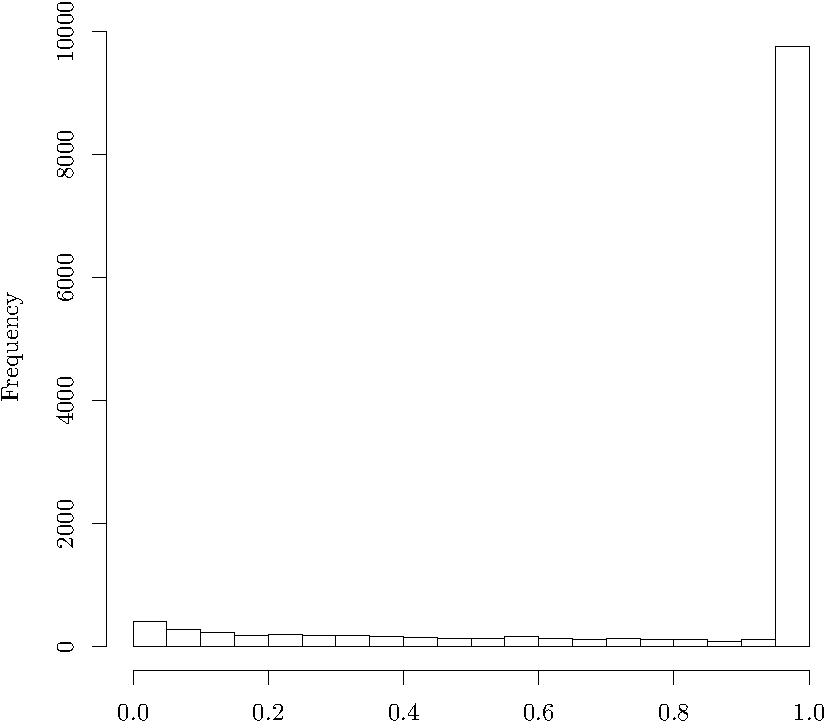
\includegraphics[width=\maxwidth]{figure/07-E3-E3-summary-3} 

}


\begin{kframe}\begin{alltt}
\hlkwd{hist}\hlstd{(}\hlkwd{log10}\hlstd{(}\hlkwd{sapply}\hlstd{(APGI.maxstat,} \hlkwa{function}\hlstd{(}\hlkwc{x}\hlstd{) x}\hlopt{$}\hlstd{p.value)),} \hlkwc{main} \hlstd{=} \hlstr{""}\hlstd{,} \hlkwc{xlab} \hlstd{=} \hlstr{""}\hlstd{)}
\end{alltt}
\end{kframe}

{\centering 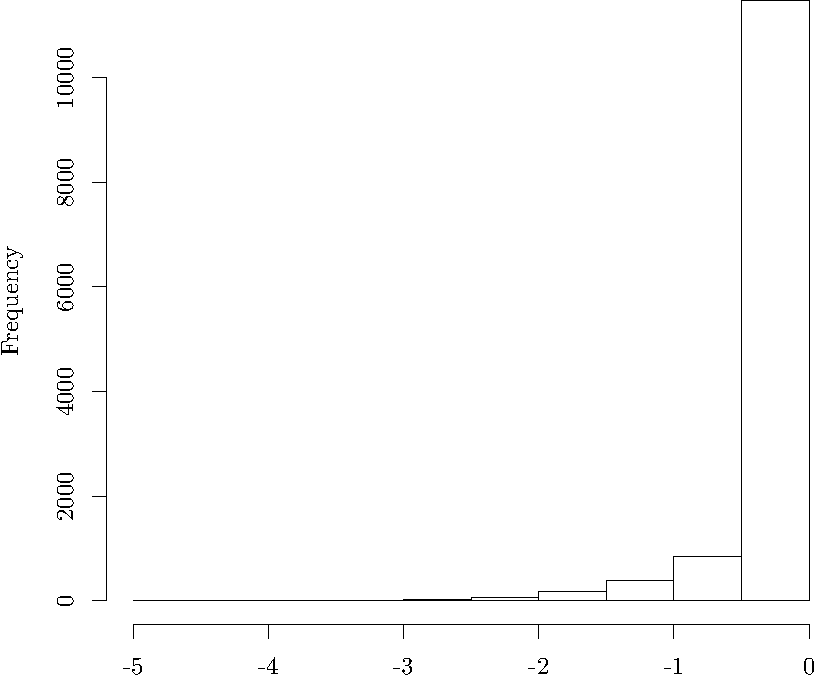
\includegraphics[width=\maxwidth]{figure/07-E3-E3-summary-4} 

}


\begin{kframe}\begin{alltt}
\hlkwd{sum}\hlstd{(}\hlkwd{sapply}\hlstd{(APGI.maxstat,} \hlkwa{function}\hlstd{(}\hlkwc{x}\hlstd{) x}\hlopt{$}\hlstd{p.value)} \hlopt{<} \hlnum{0.05}\hlstd{,} \hlkwc{na.rm} \hlstd{=} \hlnum{TRUE}\hlstd{)}
\end{alltt}
\begin{verbatim}
## [1] 413
\end{verbatim}
\begin{alltt}
\hlkwd{sum}\hlstd{(}\hlkwd{sapply}\hlstd{(APGI.maxstat,} \hlkwa{function}\hlstd{(}\hlkwc{x}\hlstd{) x}\hlopt{$}\hlstd{p.value)} \hlopt{<} \hlnum{0.05}\hlstd{,} \hlkwc{na.rm} \hlstd{=} \hlnum{TRUE}\hlstd{)} \hlopt{/} \hlkwd{length}\hlstd{(APGI.maxstat)}
\end{alltt}
\begin{verbatim}
## [1] 0.03177
\end{verbatim}
\end{kframe}
\end{knitrout}


% <<E3-plots,fig.height=4,fig.width=5,sanitize=TRUE>>=
% plot(APGI.messina, indices = 1:sum(APGI.messina@fits@summary$margin >= 1 & APGI.messina@fits@summary$passed == TRUE), sort_features = TRUE)
% plot(APGI.messina, indices = which.min(sapply(APGI.maxstat, function(x) x$p.value)), sort_features = FALSE)
% @


\begin{knitrout}
\definecolor{shadecolor}{rgb}{0.969, 0.969, 0.969}\color{fgcolor}\begin{kframe}
\begin{alltt}
\hlstd{doValidation} \hlkwb{=} \hlkwa{function}\hlstd{(}\hlkwc{train.features}\hlstd{,} \hlkwc{train.x}\hlstd{,} \hlkwc{train.threshold}\hlstd{,} \hlkwc{train.merit}\hlstd{,} \hlkwc{min_merit}\hlstd{,} \hlkwc{test.features}\hlstd{,} \hlkwc{test.x}\hlstd{,} \hlkwc{test.y}\hlstd{)}
\hlstd{\{}
        \hlkwd{require}\hlstd{(robustbase)}

        \hlstd{sel.merit} \hlkwb{=} \hlstd{train.merit} \hlopt{>=} \hlstd{min_merit}
        \hlstd{sel.val_avail} \hlkwb{=} \hlstd{train.features} \hlopt \hlstd{test.features}
        \hlstd{sel} \hlkwb{=} \hlstd{sel.merit} \hlopt{&} \hlstd{sel.val_avail}
        \hlkwd{print}\hlstd{(}\hlkwd{fisher.test}\hlstd{(}\hlkwd{table}\hlstd{(sel.merit, sel.val_avail)))}

        \hlstd{val.train.features} \hlkwb{=} \hlstd{train.features[sel]}
        \hlstd{val.train.x} \hlkwb{=} \hlstd{train.x[sel,,}\hlkwc{drop}\hlstd{=}\hlnum{FALSE}\hlstd{]}
        \hlstd{val.train.threshold} \hlkwb{=} \hlstd{train.threshold[sel]}
        \hlstd{val.train.merit} \hlkwb{=} \hlstd{train.merit[sel]}
        \hlstd{val.perm} \hlkwb{=} \hlkwd{match}\hlstd{(val.train.features, test.features)}
        \hlstd{val.test.features} \hlkwb{=} \hlstd{test.features[val.perm]}
        \hlstd{val.test.x} \hlkwb{=} \hlstd{test.x[val.perm,,}\hlkwc{drop}\hlstd{=}\hlnum{FALSE}\hlstd{]}

        \hlkwd{stopifnot}\hlstd{(val.test.features} \hlopt{==} \hlstd{val.train.features)}

        \hlcom{# Translate the threshold on the training x to an approximate equivalent}
        \hlcom{# on the test x, by normalization}
        \hlstd{locscale.train} \hlkwb{=} \hlkwd{apply}\hlstd{(val.train.x,} \hlnum{1}\hlstd{,} \hlkwa{function}\hlstd{(}\hlkwc{x}\hlstd{)} \hlkwd{scaleTau2}\hlstd{(x[}\hlopt{!}\hlkwd{is.na}\hlstd{(x)],} \hlkwc{mu.too} \hlstd{=} \hlnum{TRUE}\hlstd{))}
        \hlstd{loc.train} \hlkwb{=} \hlstd{locscale.train[}\hlnum{1}\hlstd{,]}
        \hlstd{scale.train} \hlkwb{=} \hlstd{locscale.train[}\hlnum{2}\hlstd{,]}

        \hlstd{locscale.test} \hlkwb{=} \hlkwd{apply}\hlstd{(val.test.x,} \hlnum{1}\hlstd{,} \hlkwa{function}\hlstd{(}\hlkwc{x}\hlstd{)} \hlkwd{scaleTau2}\hlstd{(x[}\hlopt{!}\hlkwd{is.na}\hlstd{(x)],} \hlkwc{mu.too} \hlstd{=} \hlnum{TRUE}\hlstd{))}
        \hlstd{loc.test} \hlkwb{=} \hlstd{locscale.test[}\hlnum{1}\hlstd{,]}
        \hlstd{scale.test} \hlkwb{=} \hlstd{locscale.test[}\hlnum{2}\hlstd{,]}

        \hlstd{val.test.threshold} \hlkwb{=} \hlstd{(val.train.threshold} \hlopt{-} \hlstd{loc.train)} \hlopt{/} \hlstd{scale.train} \hlopt{*} \hlstd{scale.test} \hlopt{+} \hlstd{loc.test}

        \hlstd{val.chisq} \hlkwb{=} \hlkwd{mapply}\hlstd{(}\hlkwa{function}\hlstd{(}\hlkwc{row_index}\hlstd{,} \hlkwc{threshold}\hlstd{) \{}
                \hlstd{x} \hlkwb{=} \hlstd{val.test.x[row_index,]}
                \hlstd{xd} \hlkwb{=} \hlstd{x} \hlopt{>} \hlstd{threshold}
                \hlkwa{if} \hlstd{(}\hlkwd{all}\hlstd{(xd)} \hlopt{||} \hlkwd{all}\hlstd{(}\hlopt{!}\hlstd{xd))        \{} \hlkwd{return}\hlstd{(}\hlnum{NA}\hlstd{) \}}
                \hlstd{fit} \hlkwb{=} \hlkwd{survdiff}\hlstd{(test.y} \hlopt{~} \hlstd{xd)}
                \hlstd{fit}\hlopt{$}\hlstd{chisq}
        \hlstd{\},} \hlnum{1}\hlopt{:}\hlkwd{length}\hlstd{(val.test.threshold), val.test.threshold)}

        \hlstd{result} \hlkwb{=} \hlkwd{data.frame}\hlstd{(}\hlkwc{merit} \hlstd{= val.train.merit,} \hlkwc{threshold.train} \hlstd{= val.train.threshold,} \hlkwc{threshold.test} \hlstd{= val.test.threshold,} \hlkwc{chisq} \hlstd{= val.chisq)}
        \hlkwd{rownames}\hlstd{(result)} \hlkwb{=} \hlstd{val.test.features}
        \hlstd{result} \hlkwb{=} \hlstd{result[}\hlkwd{order}\hlstd{(}\hlopt{-}\hlstd{result}\hlopt{$}\hlstd{merit),]}
        \hlstd{result}
\hlstd{\}}

\hlstd{val.GSE28735.messina} \hlkwb{=} \hlkwd{doValidation}\hlstd{(}\hlkwd{as.character}\hlstd{(APGI.feats}\hlopt{$}\hlstd{symbol), APGI.x, APGI.messina}\hlopt{@}\hlkwc{fits}\hlopt{@}\hlkwc{summary}\hlopt{$}\hlstd{threshold, APGI.messina}\hlopt{@}\hlkwc{fits}\hlopt{@}\hlkwc{summary}\hlopt{$}\hlstd{margin,} \hlnum{1}\hlstd{,} \hlkwd{as.character}\hlstd{(GSE28735.feats}\hlopt{$}\hlstd{Gene.symbol), GSE28735.x, GSE28735.y)}
\end{alltt}


{\ttfamily\noindent\itshape\color{messagecolor}{\#\# Loading required package: robustbase\\\#\# \\\#\# Attaching package: 'robustbase'\\\#\# \\\#\# The following object is masked from 'package:survival':\\\#\# \\\#\#\ \ \ \  heart}}\begin{verbatim}
## 
## 	Fisher's Exact Test for Count Data
## 
## data:  table(sel.merit, sel.val_avail)
## p-value = 0.003805
## alternative hypothesis: true odds ratio is not equal to 1
## 95 percent confidence interval:
##   1.552 28.453
## sample estimates:
## odds ratio 
##      6.109
\end{verbatim}
\begin{alltt}
\hlstd{val.GSE28735.maxstat} \hlkwb{=} \hlkwd{doValidation}\hlstd{(}\hlkwd{as.character}\hlstd{(APGI.feats}\hlopt{$}\hlstd{symbol), APGI.x,} \hlkwd{sapply}\hlstd{(APGI.maxstat,} \hlkwa{function}\hlstd{(}\hlkwc{x}\hlstd{) x}\hlopt{$}\hlstd{threshold),} \hlopt{-}\hlkwd{log10}\hlstd{(}\hlkwd{sapply}\hlstd{(APGI.maxstat,} \hlkwa{function}\hlstd{(}\hlkwc{x}\hlstd{) x}\hlopt{$}\hlstd{p.value)),} \hlopt{-}\hlkwd{log10}\hlstd{(}\hlnum{0.05}\hlstd{),} \hlkwd{as.character}\hlstd{(GSE28735.feats}\hlopt{$}\hlstd{Gene.symbol), GSE28735.x, GSE28735.y)}
\end{alltt}
\begin{verbatim}
## 
## 	Fisher's Exact Test for Count Data
## 
## data:  table(sel.merit, sel.val_avail)
## p-value < 2.2e-16
## alternative hypothesis: true odds ratio is not equal to 1
## 95 percent confidence interval:
##  2.431 3.653
## sample estimates:
## odds ratio 
##      2.982
\end{verbatim}
\begin{alltt}
\hlstd{val.GSE21501.messina} \hlkwb{=} \hlkwd{doValidation}\hlstd{(}\hlkwd{as.character}\hlstd{(APGI.feats}\hlopt{$}\hlstd{symbol), APGI.x, APGI.messina}\hlopt{@}\hlkwc{fits}\hlopt{@}\hlkwc{summary}\hlopt{$}\hlstd{threshold, APGI.messina}\hlopt{@}\hlkwc{fits}\hlopt{@}\hlkwc{summary}\hlopt{$}\hlstd{margin,} \hlnum{1}\hlstd{,} \hlkwd{as.character}\hlstd{(GSE21501.feats}\hlopt{$}\hlstd{Gene.symbol), GSE21501.x, GSE21501.y)}
\end{alltt}
\begin{verbatim}
## 
## 	Fisher's Exact Test for Count Data
## 
## data:  table(sel.merit, sel.val_avail)
## p-value = 1.561e-05
## alternative hypothesis: true odds ratio is not equal to 1
## 95 percent confidence interval:
##    3.835 176.208
## sample estimates:
## odds ratio 
##      18.54
\end{verbatim}
\begin{alltt}
\hlstd{val.GSE21501.maxstat} \hlkwb{=} \hlkwd{doValidation}\hlstd{(}\hlkwd{as.character}\hlstd{(APGI.feats}\hlopt{$}\hlstd{symbol), APGI.x,} \hlkwd{sapply}\hlstd{(APGI.maxstat,} \hlkwa{function}\hlstd{(}\hlkwc{x}\hlstd{) x}\hlopt{$}\hlstd{threshold),} \hlopt{-}\hlkwd{log10}\hlstd{(}\hlkwd{sapply}\hlstd{(APGI.maxstat,} \hlkwa{function}\hlstd{(}\hlkwc{x}\hlstd{) x}\hlopt{$}\hlstd{p.value)),} \hlopt{-}\hlkwd{log10}\hlstd{(}\hlnum{0.05}\hlstd{),} \hlkwd{as.character}\hlstd{(GSE21501.feats}\hlopt{$}\hlstd{Gene.symbol), GSE21501.x, GSE21501.y)}
\end{alltt}
\begin{verbatim}
## 
## 	Fisher's Exact Test for Count Data
## 
## data:  table(sel.merit, sel.val_avail)
## p-value = 1.805e-10
## alternative hypothesis: true odds ratio is not equal to 1
## 95 percent confidence interval:
##  1.649 2.540
## sample estimates:
## odds ratio 
##      2.051
\end{verbatim}
\begin{alltt}
\hlstd{val.TCGA.messina} \hlkwb{=} \hlkwd{doValidation}\hlstd{(}\hlkwd{as.character}\hlstd{(APGI.feats}\hlopt{$}\hlstd{symbol), APGI.x, APGI.messina}\hlopt{@}\hlkwc{fits}\hlopt{@}\hlkwc{summary}\hlopt{$}\hlstd{threshold, APGI.messina}\hlopt{@}\hlkwc{fits}\hlopt{@}\hlkwc{summary}\hlopt{$}\hlstd{margin,} \hlnum{1}\hlstd{,} \hlkwd{as.character}\hlstd{(TCGA.feats}\hlopt{$}\hlstd{symbol), TCGA.x, TCGA.y)}
\end{alltt}
\begin{verbatim}
## 
## 	Fisher's Exact Test for Count Data
## 
## data:  table(sel.merit, sel.val_avail)
## p-value = 1
## alternative hypothesis: true odds ratio is not equal to 1
## 95 percent confidence interval:
##  0.2236    Inf
## sample estimates:
## odds ratio 
##        Inf
\end{verbatim}
\begin{alltt}
\hlstd{val.TCGA.maxstat} \hlkwb{=} \hlkwd{doValidation}\hlstd{(}\hlkwd{as.character}\hlstd{(APGI.feats}\hlopt{$}\hlstd{symbol), APGI.x,} \hlkwd{sapply}\hlstd{(APGI.maxstat,} \hlkwa{function}\hlstd{(}\hlkwc{x}\hlstd{) x}\hlopt{$}\hlstd{threshold),} \hlopt{-}\hlkwd{log10}\hlstd{(}\hlkwd{sapply}\hlstd{(APGI.maxstat,} \hlkwa{function}\hlstd{(}\hlkwc{x}\hlstd{) x}\hlopt{$}\hlstd{p.value)),} \hlopt{-}\hlkwd{log10}\hlstd{(}\hlnum{0.05}\hlstd{),} \hlkwd{as.character}\hlstd{(TCGA.feats}\hlopt{$}\hlstd{symbol), TCGA.x, TCGA.y)}
\end{alltt}
\begin{verbatim}
## 
## 	Fisher's Exact Test for Count Data
## 
## data:  table(sel.merit, sel.val_avail)
## p-value = 0.08234
## alternative hypothesis: true odds ratio is not equal to 1
## 95 percent confidence interval:
##  0.961 2.318
## sample estimates:
## odds ratio 
##       1.46
\end{verbatim}


{\ttfamily\noindent\bfseries\color{errorcolor}{\#\# Error in if (all(xd) || all(!xd)) \{: missing value where TRUE/FALSE needed}}\begin{alltt}
\hlstd{val.GSE28735.messina}
\end{alltt}
\begin{verbatim}
##         merit threshold.train threshold.test    chisq
## KRT6A   3.999           9.503          4.754 1.638186
## ANGPTL4 2.716           8.900          3.754 0.670894
## DHRS9   1.468           8.965          4.404 0.007037
## FGG     1.365           8.585         13.796       NA
## PPY     1.098          11.931          4.068 2.536840
## LOX     1.051           7.686          6.841 0.494314
## IL20RB  1.043           6.971          4.060 0.435502
\end{verbatim}
\begin{alltt}
\hlstd{val.GSE21501.messina}
\end{alltt}
\begin{verbatim}
##         merit threshold.train threshold.test  chisq
## KRT6A   3.999           9.503         3.3849 0.2333
## ANGPTL4 2.716           8.900         0.7529 0.1246
## KRT6C   2.333           7.458        40.3387     NA
## IGFBP1  1.474           7.070        -4.0458 2.3645
## DHRS9   1.468           8.965         1.9614 3.9596
## FGG     1.365           8.585         9.7976     NA
## PPY     1.098          11.931         3.8380 0.3419
## LOX     1.051           7.686        -0.5062 0.1867
## IL20RB  1.043           6.971         1.7140 0.6682
\end{verbatim}
\begin{alltt}
\hlstd{val.GSE28735.maxstat}
\end{alltt}
\begin{verbatim}
##            merit threshold.train threshold.test     chisq
## ANGPTL4    4.835           8.356          3.527 1.217e+00
## KRT6A      4.450           8.915          4.503 2.180e+00
## LOX        4.225           7.502          6.609 5.419e-01
## PYGL       3.837           8.829          7.074 2.251e+00
## ST6GAL1    3.803           9.542          6.145 1.230e+00
## FAM189A2   3.630           6.455          4.052 3.197e-03
## KLHL5      3.511           8.978          6.464 2.728e+00
## ADM        3.394           8.820          4.730 1.088e+00
## E2F7       3.373           6.507          3.854 4.938e+00
## SMOX       3.165           7.190          4.852 2.650e-02
## KIF20A     3.123           7.250          3.584 2.396e+00
## CAPN6      3.073           6.516          4.094 7.537e-01
## IL20RB     2.994           6.505          3.492 6.901e-01
## P4HA1      2.882           9.080          7.426 3.618e-02
## FYN        2.854           8.079          6.086 5.064e-01
## AURKA      2.850           7.727          3.628 5.199e-01
## TCEA3      2.791           8.955          4.898 3.547e+00
## LOXL4      2.778           7.628          3.985 4.353e-03
## LDHA       2.744          11.922          9.716 6.056e-01
## CKAP2L     2.693           7.047          3.898 3.238e+00
## PPY        2.628          11.966          4.074 2.537e+00
## TREM1      2.588           6.546          5.146 3.641e-01
## PLOD1      2.541          10.492          5.802 6.070e-02
## CDC20      2.506           8.806          4.385 7.903e-01
## PFKP       2.483           9.183          5.636 7.701e-02
## ERRFI1     2.364          10.222          8.463 2.657e-02
## RGS5       2.303           8.665          6.941 1.157e-01
## TPX2       2.283           7.213          4.613 2.342e+00
## P4HA2      2.267           9.209          6.579 2.345e+00
## SLC15A1    2.242           6.716          5.053 4.828e-01
## DPY19L1    2.227           9.183          6.364 3.403e-02
## MME        2.227           6.441          4.645 1.425e-01
## ATF7IP2    2.212           7.139          5.793 4.623e-02
## PAEP       2.186           6.304          5.022 2.214e-01
## EPHX2      2.173           7.223          3.637 7.331e-01
## KYNU       2.169           7.161          5.370 9.540e-04
## FOXM1      2.166           6.884          4.573 5.998e+00
## NAMPT      2.159           7.988         10.049 3.699e-01
## PLOD2      2.155          10.451          7.593 3.300e+00
## UPP1       2.130           9.094          4.411 1.248e+00
## KCTD10     2.119           7.907          6.094 3.352e-04
## ZNF185     2.105           7.420          3.933 1.060e+00
## EDIL3      2.105           6.400          8.217 5.409e-03
## NEK2       2.103           8.167          4.426 5.032e-01
## LCP1       2.100           8.702          6.629 6.413e+00
## GAPDH      2.086          11.336          9.814 1.951e+00
## ARSD       2.085           9.970          6.440 2.866e+00
## KIF2C      2.080           6.839          3.953 3.629e+00
## ENO2       2.069           7.557          5.422 3.748e-02
## COL12A1    2.052           8.689          8.314 5.723e-02
## VSNL1      2.052           6.712          4.221 2.337e-03
## ENTHD1     2.044           6.345          3.130 1.851e-01
## CADPS2     2.043           7.892          5.795 3.026e+00
## ASPM       1.993           7.916          5.271 9.366e-02
## ASAP1      1.993           9.917          7.260 4.509e-02
## SPATA18    1.952           7.197          5.264 2.207e+00
## KRT18      1.943          12.487          7.917 6.325e-01
## POLQ       1.938           6.758          3.609 5.093e+00
## FAM3D      1.933           9.474          6.136 2.076e+00
## CD109      1.929           6.370          5.959 2.207e-01
## UBE2C      1.927           9.305          5.228 1.843e+00
## OCLN       1.922           7.722          7.186 5.277e-01
## WNK2       1.915           6.293          3.922 2.774e+00
## TGFBI      1.912          12.180          8.229 2.750e+00
## SPOCK1     1.903           8.915          5.387 7.009e+00
## CD300A     1.885           6.707          5.248 1.331e-01
## RAVER2     1.856           7.583          5.856 7.799e-01
## P2RY8      1.856           7.349          4.024 1.079e-02
## A4GNT      1.846           6.439          3.549 1.023e+00
## RIMKLB     1.825           7.221          6.093 7.238e-03
## ADAM23     1.824           6.394          4.155 7.598e-03
## FST        1.820           7.155          4.557 1.088e+00
## CA8        1.819           6.429          3.264 1.650e+00
## CEP55      1.819           7.985          4.831 1.431e+00
## IL1A       1.813           6.266          2.599 1.460e-01
## ANLN       1.811           7.020          4.871 3.439e+00
## DCBLD2     1.806          10.689          8.544 7.788e+00
## PLA2G10    1.795           9.726          4.000 4.374e+00
## KLHL13     1.791           6.430          3.543 6.677e-01
## STAG3L4    1.784           6.532          4.970 3.087e-01
## GOLM1      1.777           6.547          8.986        NA
## F3         1.770           9.228          7.930 4.135e-02
## NTS        1.760           6.317          2.643 1.702e+00
## TPI1       1.759          10.890          6.342 4.913e-01
## PTGES      1.757           7.540          4.722 7.838e-06
## IGKV1ORY-1 1.755          11.809          7.375 2.201e-03
## SNAI2      1.753           8.469          6.705 7.687e-02
## NFIA       1.727           7.914          5.845 1.255e+00
## COL7A1     1.726           8.066          4.932 2.645e+00
## FGD6       1.724           6.426          6.617 9.292e-01
## MCM4       1.721           7.948          5.209 1.214e+00
## TUBA1C     1.720          11.899          6.920 1.285e-02
## MELK       1.713           7.288          4.752 2.117e+00
## C5orf46    1.700           6.858          2.836        NA
## COL17A1    1.700          10.742          6.042 7.886e-01
## PDLIM7     1.691           8.030          6.383 6.057e-01
## PTTG1      1.674           9.067          4.939 1.004e+00
## DSG2       1.663          10.999          7.174 6.084e+00
## COL1A2     1.658          12.989         11.330 1.470e+00
## SYNE2      1.657           8.782          7.637 1.589e-01
## SERPINH1   1.646          10.187          6.735 2.134e+00
## PHLDA1     1.643           9.269          6.348 1.132e+00
## CTSE       1.642          11.677          9.666 1.154e+00
## ADH1A      1.635           8.432          4.306 3.482e+00
## WEE1       1.635           7.480          7.084 1.675e+00
## CHEK1      1.623           6.501          4.403 2.718e+00
## GSDMC      1.618           6.409          3.565 4.329e+00
## SLC2A1     1.615          10.218          7.422 3.749e-03
## SERPINB3   1.614           6.324          2.770 1.020e-02
## DHRS9      1.609           8.430          4.046 2.091e-01
## PPP1R3C    1.597           8.282          5.976 3.812e+00
## FLRT3      1.596           9.224          5.713 3.404e+00
## CCNB2      1.594           7.685          4.108 1.338e+00
## CORO1A     1.593           8.375          5.960 4.792e-03
## RHOF       1.591           6.800          4.881 5.617e-01
## GRAMD3     1.587           7.707          5.612 7.763e-03
## IL33       1.583           7.299          4.397 2.122e-03
## AQP1       1.577           7.146          5.848 7.817e-02
## VEGFA      1.573           7.090          6.212 1.095e-02
## ANGPTL2    1.563           9.897          5.866 1.308e+00
## SEMA4A     1.562           7.304          4.697 1.226e-01
## GCNT1      1.562           8.263          6.462 2.802e-01
## CCL19      1.560           9.155          6.111 2.032e-01
## CACHD1     1.555           6.709          5.075 4.289e-03
## NCAPG      1.544           7.323          5.149 4.495e-01
## FCGR2B     1.536           7.007          4.506 2.784e-02
## BOC        1.528           6.805          5.509 3.207e+00
## CNIH3      1.513           6.461          4.149 9.764e-01
## IL1R2      1.508           8.252          5.522 3.305e+00
## ITGA5      1.505           8.100          5.330 7.701e-02
## ITM2A      1.504           9.660          5.222 7.935e-01
## SLC9A9     1.502           7.348          6.777 2.790e-02
## TM4SF19    1.496           6.269          4.532 1.245e+00
## JAG1       1.488           9.130          8.263 4.872e+00
## FN1        1.486           6.406         11.169 2.450e-02
## NRP2       1.484           6.606          8.615        NA
## TNNI2      1.480           6.303          4.497 3.223e-01
## APOL1      1.469           6.456          7.103 6.062e-02
## KANK4      1.468           7.979          4.247 2.105e-01
## RFX2       1.463           6.427          5.086 5.510e-01
## DSC2       1.458           6.704          7.468 8.154e+00
## KRT17      1.449          10.862          6.923 1.492e+00
## ANKLE2     1.448           7.795          6.781 1.866e+00
## PRC1       1.445           8.324          5.413 2.803e+00
## PPP2R2C    1.443           6.859          3.662 4.825e+00
## KIF18A     1.440           6.472          3.550 1.717e+00
## NDRG2      1.438           8.691          6.250 2.768e+00
## LONRF2     1.437           6.411          4.445 4.865e-01
## SEMA3A     1.432           7.328          6.924 1.541e+00
## ARHGAP26   1.426           6.622          7.091 3.126e+00
## ZBED2      1.424           6.267          4.047 1.361e+00
## PCF11      1.422           6.970          5.972 5.690e+00
## IGJ        1.420           9.761         10.380 1.711e-02
## RGS16      1.419           6.813          5.669 4.387e+00
## HRASLS2    1.418           7.346          3.576 1.641e-01
## AHCYL2     1.417           8.620          7.190 4.483e+00
## TLE4       1.417           8.089          5.644 1.763e-02
## CDA        1.416           6.859          4.461 1.855e-01
## DNASE1     1.415           6.346          3.864 6.021e-01
## DKK1       1.413           9.728          5.287 1.032e+00
## CD38       1.405           7.104          6.298 7.484e-01
## MALL       1.405          10.388          6.245 3.778e-01
## GIMAP2     1.400           7.313          5.276 2.303e+00
## GPC3       1.399           7.457          6.106 8.675e-01
## SH3RF1     1.391           8.535          6.363 4.798e+00
## DUOXA2     1.384           7.261          4.065 3.746e+00
## FRMD6      1.379           9.411          7.018 1.674e+00
## KNTC1      1.365           7.209          5.133 2.333e+00
## TMSB10     1.364          13.721         10.239 9.794e-01
## KPNA2      1.356           6.543          6.121 6.968e-01
## CST6       1.354           8.451          4.027 1.272e+00
## CCNB1      1.353           7.364          5.563 3.176e-01
## CD79A      1.350           7.991          4.204 1.653e+00
## RAP1GAP    1.346           9.590          3.821 2.320e-01
## CENPF      1.346           7.209          5.142 5.130e-01
## SOD2       1.341           8.755          7.349        NA
## MIF        1.334          12.328          7.195 2.992e-01
## GBE1       1.331           7.564          6.499 1.296e+00
## MEOX1      1.331           6.748          4.334 3.263e-02
## KIF14      1.322           6.914          3.835 3.222e+00
## TRNP1      1.319          10.665          5.963 4.984e-03
## FGG        1.319           8.010         10.996        NA
## MUC16      1.312           6.930          3.937 1.296e-01
## DYNC2H1    1.312           7.510          6.309 4.117e+00
## MMP10      1.307           6.412          2.984 6.057e-01
## LETM2      1.306           6.642          4.413 6.681e-01
\end{verbatim}
\begin{alltt}
\hlstd{val.GSE21501.maxstat}
\end{alltt}
\begin{verbatim}
##          merit threshold.train threshold.test     chisq
## ANGPTL4  4.835           8.356        0.19587 6.865e-01
## KRT6A    4.450           8.915        2.97484 2.615e-02
## LOX      4.225           7.502       -0.79221 1.058e+00
## KRT6C    4.215           6.392        5.59238        NA
## ST6GAL1  3.803           9.542        0.78319 5.739e-01
## FAM189A2 3.630           6.455        0.28808 7.248e-01
## ADM      3.394           8.820       -1.66023 7.681e+00
## E2F7     3.373           6.507       -2.26972 1.101e+01
## CAPN6    3.073           6.516        0.58777 1.934e+00
## IL20RB   2.994           6.505        0.27819 2.890e+00
## FGF13    2.837           6.400       -0.33980 2.197e+00
## TCEA3    2.791           8.955        0.67789 4.561e+00
## LOXL4    2.778           7.628        0.96728 4.499e-01
## TMEM26   2.688           6.692        0.77037 4.695e-02
## BIRC5    2.643           7.334       -1.61111 4.021e+00
## CD70     2.632           6.748       -0.60306 5.035e-01
## PPY      2.628          11.966        3.85564 7.804e-01
## TREM1    2.588           6.546        2.12235 4.167e+00
## IGFBP1   2.466           7.076       -4.02812 1.675e+00
## ERRFI1   2.364          10.222        0.59119 1.790e+01
## RGS5     2.303           8.665        4.26999 5.369e+00
## PHACTR3  2.275           6.884        1.98393 1.343e+00
## MME      2.227           6.441       -1.58576 2.189e-01
## PRDM16   2.206           6.605        3.97296 1.839e+00
## PAEP     2.186           6.304        0.77117 4.242e-01
## EPHX2    2.173           7.223        0.03016 4.564e-01
## KYNU     2.169           7.161       -1.99673 3.795e-01
## NAMPT    2.159           7.988        0.11528 1.970e+00
## PLOD2    2.155          10.451        0.06961 8.655e-02
## EDIL3    2.105           6.400        4.24471 1.304e+00
## NEK2     2.103           8.167       -1.80395 4.750e+00
## LCP1     2.100           8.702       -1.84614 2.896e+00
## COL12A1  2.052           8.689        1.83301 3.053e-01
## VSNL1    2.052           6.712       -1.64740 1.529e-01
## ENTHD1   2.044           6.345        1.75682 2.632e-01
## PCDH20   2.003           7.551        3.99419 1.354e+00
## ASPM     1.993           7.916       -0.07079 1.759e+00
## CATSPER1 1.956           6.371        0.89696 1.486e+00
## KRT18    1.943          12.487        0.25249 1.552e+00
## FAM3D    1.933           9.474        5.30834 6.346e+00
## CD109    1.929           6.370       -0.49431 4.737e-01
## UBE2C    1.927           9.305       -1.15748 2.006e+00
## OCLN     1.922           7.722        2.27334 3.056e+00
## TGFBI    1.912          12.180        1.17508 7.810e-02
## SPOCK1   1.903           8.915       -0.07385 3.241e-02
## P2RY2    1.899           6.885        2.53729 5.626e-01
## RAVER2   1.856           7.583        0.05711 4.701e-01
## P2RY8    1.856           7.349        0.52845 1.882e+00
## A4GNT    1.846           6.439        3.40057 8.431e-01
## APOA4    1.823           6.333       -1.04560 3.747e-01
## CEP55    1.819           7.985       -0.77283 1.442e-03
## IL1A     1.813           6.266       -0.13329 2.483e-02
## ANLN     1.811           7.020       -2.66571 1.547e-01
## DCBLD2   1.806          10.689        0.63766 4.607e+00
## PLA2G10  1.795           9.726        3.52033 1.519e-01
## GOLM1    1.777           6.547        4.36321 3.484e+00
## F3       1.770           9.228        3.33470 7.961e-01
## NTS      1.760           6.317       -5.02906 1.450e+00
## SNAI2    1.753           8.469        0.96462 2.333e+00
## COL7A1   1.726           8.066       -0.65725 1.243e+00
## FGD6     1.724           6.426        1.00560 2.874e-02
## NFIX     1.713           9.904        1.57937 1.036e+00
## C5orf46  1.700           6.858        1.16807 5.466e+00
## COL17A1  1.700          10.742        4.24593 2.682e-01
## VSTM2L   1.679           7.078        2.67464 2.975e-01
## COL1A2   1.658          12.989        3.96788 4.629e-03
## SERPINH1 1.646          10.187        0.16779 4.575e+00
## CTSE     1.642          11.677        7.26038 3.184e+00
## TNFRSF6B 1.638           7.634        3.32680 6.004e-01
## ADH1A    1.635           8.432        2.32552 1.282e+00
## CHEK1    1.623           6.501       -3.47669 7.154e-02
## SLC2A1   1.615          10.218       -0.52907 5.130e-01
## SERPINB3 1.614           6.324        0.71096 4.767e-01
## DHRS9    1.609           8.430        1.56562 2.307e+00
## PPP1R3C  1.597           8.282        0.52826 8.428e-05
## FLRT3    1.596           9.224        3.15856 2.789e+00
## CCNB2    1.594           7.685       -0.56249 1.099e+00
## CXCR5    1.589           6.681        7.98854        NA
## IL33     1.583           7.299        4.11799 2.212e-02
## AQP1     1.577           7.146        3.32621 1.330e-01
## TNFRSF17 1.573           7.032       12.81828        NA
## VEGFA    1.573           7.090       -0.39754 2.750e-01
## GCNT1    1.562           8.263        1.40450 6.109e-02
## CCL19    1.560           9.155        5.98546 9.945e-01
## ADRA1B   1.546           6.285        0.12758 3.060e+00
## CAV2     1.540           8.562        1.61441 2.749e+00
## FCGR2B   1.536           7.007        1.56740 9.048e-01
## MRAP2    1.532           7.684        0.29126 2.912e-01
## CCL3L3   1.524           6.799        1.79960 1.696e+00
## CNIH3    1.513           6.461        0.57543 1.041e+00
## IL1R2    1.508           8.252        3.85019 2.006e-01
## ITM2A    1.504           9.660       -0.78323 1.336e+00
## SLC9A9   1.502           7.348        3.46665 9.579e-02
## FN1      1.486           6.406        0.04531 3.830e-01
## SOX8     1.486           7.496        0.79012 5.370e-03
## NRP2     1.484           6.606        5.28797        NA
## TNNI2    1.480           6.303       -1.30119 7.253e+00
## HES1     1.479           8.112        1.10294 4.000e-01
## KCNH2    1.476           6.778        0.69336 2.375e+00
## APOL1    1.469           6.456        0.79884 2.381e-02
## KANK4    1.468           7.979        1.54307 1.052e-01
## KRT17    1.449          10.862        1.84873 3.034e+00
## PPP2R2C  1.443           6.859       -0.11054 1.115e-01
## KIF18A   1.440           6.472       -2.19452 1.770e-01
## LONRF2   1.437           6.411       -1.25358 1.612e+00
## SEMA3A   1.432           7.328        0.13548 6.067e-01
## ARHGAP26 1.426           6.622        1.86500 5.095e-01
## ZBED2    1.424           6.267        2.24266 7.387e-01
## SPOCD1   1.422           6.904        1.25823 5.807e+00
## IGJ      1.420           9.761        1.21379 3.078e-01
## RGS16    1.419           6.813        1.94034 2.366e-01
## HRASLS2  1.418           7.346        4.41621 2.843e-01
## AHCYL2   1.417           8.620        1.74374 4.884e+00
## DNASE1   1.415           6.346        0.03199 5.313e-02
## DKK1     1.413           9.728        0.52018 1.947e+00
## CD38     1.405           7.104        2.18938 7.635e-01
## MALL     1.405          10.388        3.83833 5.231e-01
## FGF18    1.397           6.280        1.94601 3.342e-03
## ZNF365   1.390           7.180        2.32667 3.166e-01
## FRMD6    1.379           9.411        1.01822 1.170e-02
## TK1      1.375           8.114       -1.37859 4.348e+00
## CST6     1.354           8.451        4.65564 2.530e-01
## CD79A    1.350           7.991        2.33695 7.925e-02
## RAP1GAP  1.346           9.590        0.53578 8.878e-03
## CENPF    1.346           7.209       -2.07887 2.536e+00
## SOD2     1.341           8.755       -0.40747 6.928e-01
## MEOX1    1.331           6.748        0.96369 5.732e-01
## KIF14    1.322           6.914       -1.85459 3.210e-01
## TRNP1    1.319          10.665        3.20514 9.527e-04
## FGG      1.319           8.010        6.42581        NA
## CBX1     1.317           6.644        0.09649 4.679e-01
## MUC16    1.312           6.930       -1.13833 1.513e-01
## DYNC2H1  1.312           7.510        0.47423 6.089e-03
## GATA6    1.310           6.470        3.72622 2.664e+00
## MMP10    1.307           6.412        1.44298 3.202e-02
\end{verbatim}
\begin{alltt}
\hlstd{val.TCGA.messina}
\end{alltt}
\begin{verbatim}
##         merit threshold.train threshold.test  chisq
## KRT6A   3.999           9.503          3.656 1.4483
## ANGPTL4 2.716           8.900          3.336 0.2310
## KRT6C   2.333           7.458         16.773     NA
## CIDEC   2.269           8.021          3.192 2.0245
## IGFBP1  1.474           7.070          3.788     NA
## DHRS9   1.468           8.965          3.203 0.1557
## FGG     1.365           8.585         10.219     NA
## LYNX1   1.344           7.020          3.998     NA
## PPY     1.098          11.931          3.969 0.3139
## LOX     1.051           7.686          3.602 0.3011
## IL20RB  1.043           6.971          2.975 4.0928
\end{verbatim}
\begin{alltt}
\hlstd{val.TCGA.maxstat}
\end{alltt}


{\ttfamily\noindent\bfseries\color{errorcolor}{\#\# Error in eval(expr, envir, enclos): object 'val.TCGA.maxstat' not found}}\end{kframe}
\end{knitrout}

\end{document}
